This chapter introduces techniques of solving evolution equations
for physical systems with the help of a computer.
After an introduction,
a basic review of the literature, standard definitions and techniques
is given. The focus is then turned to the codes used
or developed within this work. Note that this chapter is with a slight
focus on relativistic theories (in astrophysics), but kept technical and
general. In contrast, chapter \ref{chapter:gr} is devoted to the
Einstein equations and chapter \ref{chapter:hydro} to hydrodynamics,
where the actual equations are discussed in detail.

The results of this chapter have been published in
\cite{Dumbser2017,Fambri2018,Koeppel2017,exahype-review} and texts
in this chapter are partially based on these publications.

\section{Motivation: Hamiltonian time 
evolution}\label{sec:hamiltonian-motivation}
The broad class of ``evolution equations'' can be motivated
by Hamiltonian dynamics: Given a 
Hamiltonian system, the Hamiltonian $H$ allows to predict the value of
any function $f=f(q,p,t)$ of canonical coordinates $q,p$ and time $t$,
once $f_0=f(q,p,t_0)$ is known at an initial time $t_0$.
This can be written as
\begin{equation}\label{eq:intro.hamiltonian}
\pp ft = \left\{ f, H \right\}
= \pp fq \pp Hp - \pp fp \pp Hq
\end{equation}
where the curly brackets indicate the Poisson bracket and the equation
itself is a way to write Liouville's theorem which holds for a broad class
of physical theories such as classical mechanics and quantum mechanics,
where at the latter, the Poisson brackets are replaced by the canonical
commutator and equation \eqref{eq:intro.hamiltonian} gets an abstract
Schroedinger equation $\partial_f = [f,H]$ \footnote{
	In fact, Chapter~\vref{chapter:qgr} deals with modifying this
	commutator in order to introduce quantum effects into GR without
	doing canonical quantization.
	% Still: (Ref: QFT for Mathematicans)
}.

The Hamiltonian equations of motion
$\{ \dot q=\partial_p H, \dot p=-\partial_q H\}$ can be written as a
flux conservative evolution law
\footnote{We use Einstein sum convention, repeated indices are summed over.}
\begin{equation}\label{sec:intro-hamilton-flux}
\partial_t Q^k = \partial_i F^{ik}(Q)
\end{equation}
for the two-dimensional phase space coordinate $\vec Q=(p,q)$ with gradient 
vector $\vec \partial=(\partial_p, \partial_q)$ and $2\times2$ flux matrix
$F^{ik}=\epsilon^{ik} H(Q)$ determined by the Hamiltonian
$H=H(q,p,t)$ of the system\footnote{
  With $\epsilon^{ik}$ the Levi civita symbol in two dimensions
  (Appendix \vref{apx:symbols}).  
  Note that in this chapter, the position of indices has no
  physical meaning
  (no covariant/contravariant tensors involved).
}. 

The Hamil\-ton-Jacobi equation \eqref{eq:intro.hamiltonian} can be written as
$\partial_t f = \dot {Q_i}\partial^i f = \partial_i \dot  Q^i f$ since
$\partial_i Q^i=0$. This gives
rise to also write it in flux conservative form \eqref{sec:intro-hamilton-flux},
with an extended
\begin{equation}
\text{solution vector}~\tilde Q=(\dot Q, f)
~\text{and fluxes}~\tilde F=\begin{pmatrix}
 F^{ik} & 0 \\ 0 & \dot Q f
\end{pmatrix}\,.
\end{equation}
%solution vector $\tilde Q=(\dot Q, f)=(\dot p,\dot q, f)$ and
%fluxes $\tilde F=\operatorname{diag}(F, \dot Q f)$.
This conservation law 
rewrite exposes the
conservation of $f$ in phase space  and gives rise to a probability
distribution interpretation of $f$. 

%
%Leaving quantum mechanics aside,
%% quantumness is not covered at all in this work,
%the Cauchy initial value formulation as the canonical answer within (general)
%relativity to the ambiguity of time in four dimensional spacetime will be the
%groundwork of time evolutions in GR (Chapter \ref{chapter:gr}) and fluid
%dynamics (Chapter \ref{chapter:hydro}). It is fair to say that, in general,
%the \emph{time} evolution is actually an evolution into a direction%
%\footnote{In this chapter \ref{chapter:numerics}, the (syntactical) 
%lower/upper position of an index has no (semantic) meaning, as the concept
%of covariant and contravariant vectors has no relevance here.}
%$x^i$ where
%the system's solution at $x^i < x_0$ is known and $x^i > x_0$ shall be 
%%%predicted,
%where the solution at $x_0$ is the basis for the \emph{initial value problem}
%(IVP).

%\subsection{The meaning of time}
It is worth mentioning that in the mathematical initial value boundary problem,
\emph{time} is a name for the evolution direction and gets its semantic
meaning only in physics\footnote{
	Section~\vref{sec:adm} provides another discussion of \emph{time} in the
	Cauchy initial value formulation of general relativity.
}.
Ultimately, a ``time evolution'' is an \emph{extension} from the boundary $t_0$
of a known domain, characterized by $t < t_0$, into an unknown domain $t > t_0$.
An example where the evolution direction is not called time is the adoption
of the Cauchy-Riemann equations,
\footnote{an introductory example from \cite{Toro99}}
\begin{equation}\label{sec:intro.cauchy-riemann}
\partial_ x u = \partial_y v
\,,\quad\quad \partial_y u = - \partial_x v
\,,
\end{equation}
to perform an analytic continuation of a complex function
$f(x,y)=u(x,y) + i\,v(x,y)$, with $z=x+iy$, from the real numbers to the
complex domain. Then one can recast the imaginary axis as time, $t=y$, and write
the PDE in flux conservative form $\partial_t Q_k = \partial_x F_k$
as a time evolution of $Q_k$ in one-dimensional space ($x$), with
state $Q=(u,v)$ and fluxes $F=(-v, u)$. As both the flux $F$ and the function 
$f$ are linear in $Q$, a holomorphic function (\ie a solution to 
\eqref{sec:intro.cauchy-riemann}) is conserved within analytic continuation.
%

\section{Conservation laws}\label{sec:conservation-laws}
A general definition of a conservation law is
\begin{equation}\label{intro:conservation-law}
\partial_t u_k + \partial_i F^i_k(u) = 0
\end{equation}
and we call $\vec u=\vec u(t, \vec x) \in \mathbb R^n$ the conserved quantity or
(system) state, $\vec \partial \in \mathbb R^d$ is the vector differential operator
(Nabla operator) in $d$ spatial dimensions. $\vec F_k$ is called the \emph{flux} for 
$u_k$, all fluxes $F^i_k \in \mathbb R^{d\times n}$ together
encode the physical evolution law\footnote{
  All quantities introduced here should be understood as \emph{fields}
  $\phi=\phi(t,\vec x)$, and therefore $F(u)$ only has an implicit
  dependence on time and location. However, one can triviall make this dependence
  explicit by including the coordinates $\vec x$ itself into the state vector.
}.

$\vec u$ is frequently refered to as \emph{state vector}, but in general no
transformation properties as for a vector in physics are required within
this chapter, and for the theories presented in this work, $\vec u$ will not
transform as a vector inphysics. Instead, this object should be
refered to as the \emph{state tuple} of length $n\in\mathbb N$. While for
conservation
laws the distributional interpretation of $\vec u$ suggests $u_i\in\mathbb R$,
in general there is nothing prohibiting one from unsing alternative spaces,
such as a complex state vector $u_i \in \mathbb C$, as well as elements $u_i$ 
following any other transformation rule\footnote{
	For instance a state vector holding square matrix elements
	$u_i = m_{kj} \in M^{N\times N}(\mathbb R)$,
	with the row-major sequentialization rule $i=f(k,j)=Ni+j$.
}. In these cases, the state vector should collect all \emph{degrees of freedom}
of the mathematical objects it holds. Sometimes, \eqref{intro:conservation-law}
is written compactly in spacetime as $\partial_u F^\mu_k(u)=0$, and $F^0_k(u)$
then allows to map $u$ to the mathematical objects of interest.

\subsection{The non-conservative product}\label{sec:ncp}
If one allows an arbitrary (differential) source term $\vec{\mathcal S}=\vec{\mathcal{S}}(u, 
\partial_i u)$\footnote{
	In this section, we restrict on first order theories, so any higher order
	derivatives of $u$ are neglected.
} to add sinks and
sources for $\vec u$, the resulting modification of 
\eqref{intro:conservation-law} is called a \emph{balance law},
\begin{equation}\label{intro:balance-law}
\partial_t u_k + \partial_i F^i_k(u) = \mathcal S_k(u, \partial_i u) \,.
\end{equation}
Sources are a convenient way to formalize the coupling to other theories,
however if a source term depends on derivatives of $u$,
the differential seperability of the balance law and an external theory is
questionable. In order to formalize the differential structure of the
PDE in question, the arbitrary source term $\mathcal S_k$ shall be restricted
to an \emph{purely algebraic source term} $S_k=S_k(u)$. Instead, derivatives
shall be collected in another in an explicit quasi-linear nonconservative term which
couples to the gradient field of $u$, giving rise to a modified balance 
law
%\footnote{
% It is in fact by intention to formalize allways how derivatives can enter
% the PDE system, \ie not to just write $\partial_t u + \mathcal R(u,\partial_i 
%u) = 0$ with a differential operator $\mathcal R$.
% The reason for that is that the schemes presented in the next sections,
% such as in the Riemann solver presented in \cite{DumbserToro2011}. 
%}
\begin{equation}\label{intro:ncp}
\partial_t u_k + \partial_i F^i_k(u) + B^{ij}_k(u) \partial_i u_j = S_k(u)
\end{equation}
We refer to $B^j_k \in R^{n\times n}$ as the non-conservative matrices%
\footnote{To avoid confusion, all indices are given in equation
\eqref{intro:ncp}. However, again, the index position has \emph{no} meaning
in terms of contra/covariant. In three dimensions, $B=(B^{1a}_b,B^{2a}_b,B^{3a}_b)$
is a vector of three $R^{n\times n}$ matrices. The same applies for
the system matrices $A^i$ introduced in \eqref{intro:quasi-linear}.
}
and to $B^i(u) \partial_i u$ as the non-conservative product (NCP) or the
non-conservative flux (in contrast to the conservative flux).

The advantage of introducing the non-conservative product is that it can be
straightforwardly included in the quasi-linear formulation (next section) and in numerical
methods (Section~\ref{sec:riemann-nonconservative} goes into detail about
the inclusion in a Riemann solver).

\subsection[Quasi-linear PDEs]{Quasi-linear PDEs and 
their eigensystem}\label{sec:intro-eigensystems}
All evolution laws presented so far are first order partial differential
equations (PDEs). There is a rich theory of this class of PDEs, based on
casting the PDE as a quasi linear system
\begin{equation}\label{intro:quasi-linear}
\partial_t u_k + A^{ij}_k(u) \partial_i u_j = S_k(u)
\end{equation}
with the $d$ system matrices $A^i\in\mathrm R^{n\times n}$ given by
\begin{equation}
A^i = A^{ij}_k(u) = \partial F^i_k(u) / \partial u_k + B^{ij}_k(u)
\end{equation}
and sometimes also called velocity matrices.
The theory of hyperbolic PDEs investigates the system matrixes $A^i$ in an
eigenvalue analysis. Therefore, the \emph{differential} contributions to 
\eqref{intro:quasi-linear} are recognized as part of a \emph{differentially} linear system
\footnote{
  That means especially that the purely algebraic sources $S$ do not contribute
  to the characteristic form.
  %Causally speaking, $S$ provides no
  %differential contribution ($\d S=0$).
}.
In the eigenbasis, the system decouples to $n$ advection equations of type
$\partial_t \phi_k + \lambda_k \partial_i \phi_k = 0$, where $\phi_k$ are
called the characteristic fields. The eigenvalues $\lambda_k$ are 
recognized as the fundamental propagation speeds of waves in
a hyperbolic system. \footnote{see for instance classical textbooks about 
hyperbolic systems \cite{Toro99,Leveque92}}

Higher order PDEs have to be rewritten to first order to reveal their
characteristic structure. A classic example is the one dimensional wave equation~\cite{Toro99}
\begin{equation}
\partial_t^2 \phi - c^2 \partial_x^2 \phi = 0
\end{equation}
which is trivially rewritten as two first order equations, by means of factorizing
the differential operator
\begin{equation}
\left( \partial_t - c \partial_x \right)
\underbrace{ \left( \partial_t + c \partial_x \right) \phi }_{:= \psi}
= 0 \,,
\end{equation}
where the auxilliary field $\psi$ was introduced
and a set of two couple PDEs is obtained,
\begin{equation}\label{eq.intro.waveeq.firstorder}
\partial_t \psi - c \partial_x \psi = 0
\,,\quad
\partial_t \phi + c \partial_x \phi = \psi
\,.
\end{equation}
The first order in time and space formulation of the wave equation 
\eqref{eq.intro.waveeq.firstorder} can then be brought into quasi-linear
form \eqref{intro:quasi-linear} and then immediately exposes the wave speeds
$\pm c$, since $A^x$ is diagonal,
\begin{equation}\label{eq.intro.waveeq.A}
\partial_t
\begin{pmatrix} \psi \\ \phi \end{pmatrix}
+
\underbrace{
\begin{pmatrix} -c & 0 \\ 0 & +c  \end{pmatrix}
}_{A^x}
\partial_x
\begin{pmatrix} \psi \\ \phi \end{pmatrix}
= 
\begin{pmatrix} 0 \\ \psi \end{pmatrix}
\,.
\end{equation}%

\begin{marginfigure}[10cm]
	\begin{tikzpicture}[node distance=1cm]
	\node (A) {$A$};
	\node[below=of A] (hyperbolic) {hyperbolic}
	edge[<-] (A.south); 
	\node[left=0.2cm of hyperbolic] (parabolic) {parabolic}
	edge[<-] (A.south); 
	\node[right=0.2cm of hyperbolic] (elliptic) {elliptic}
	edge[<-] (A.south);
	
	\node[below=of hyperbolic] (strongly) {strongly}
	edge[<-] (hyperbolic.south);
	\node[right=0.5cm of strongly] (weakly) {weakly}
	edge[<-] (hyperbolic.south);
	
	\node[below=1cm of strongly] (strictly) {strictly}
	edge[<-] (strongly);
	
	\node[below=of strictly] (symmetric) {symmetric}
	edge[<-] (strictly);
	\end{tikzpicture}
	\caption[
	PDE standard classification, TikZ figure, \exclusive
	]{Standard classification of (first order) PDE systems depending
		n the system matrix $A$. The relationship $x \to y$ means
		that each $y$ has also all properties of $x$ (ie. each $y$
		is a $x$), but not the other way around.
		}%
	\label{fig:intro-pde-classification}
\end{marginfigure}%

Depending on the eigenvalues of $A^i$, the PDE system is called
elliptic (not a single real eigenvalue, an example is the Poission equation
$\partial_i\partial^i u = f$ where the wave speeds are unlimited),
parabolic (an example is the heat equation $\partial_t u - \alpha 
\partial_i\partial^i u=0$)
or hyperbolic ($n$ real eigenvalues, as the presented wave equation
\eqref{eq.intro.waveeq.firstorder}). Weak hyperbolicity is given if the
set of eigenvectors is not complete (\ie $A^i$ not diagonalizable),
while strong hyperbolicity is given with a complete set of eigenvectors
(and real eigenvalues).
Strict hyperbolicity is given with $n$ distinct eigenvalues.
Symmetric hyperbolicity is given when $A^i$ is symmetric and thus diagonalizable
(see Figure~\ref{fig:intro-pde-classification} for a diagram). In one
spatial dimension, all strongly hyperbolic systems are also symmetric 
hyperbolic.

Weakly hyperbolic PDEs suffer from well-posedness, \ie small perturbations 
in the initial data can change the solution dramatically
(Appendix \ref{sec:apx-pde-classification}). In contrast, strongly hyperbolic 
systems
can be decomposed into independent advection equations (characteristics) with
the help of a symmetrizer matrix which is composed by the (right) eigenvectors.
The different finite wave speeds of the characteristics are given by the eigenvalues of
the system matrix, which accounts for the wave-like nature associated with
hyperbolic systems.

\emph{Stiffness} is another feature which can be derived from the eigenstructure:
PDEs which describe phenomena on very different timescales. Stiffness is defined 
by the ratio $R=\lambda_\text{max}/\lambda_\text{min}$ between the largest and the
smallest eigenvalue (wave speed), and a large stiffness $R\gg 1$ can be challenging
for a computer-aided solution.

For linear PDEs, where $A^i(u) = A^i$ does not depend on the state $u$ and thus the
quasi-linear form is also algebraically linear, any PDE can be
reduced to ordinary differential equations (ODEs) by separation of variables.
For nonlinear systems, fundamental definitions of existence and uniqueness of a
solution to the PDE must be solved. A popular example are the harmonic solutions
of Laplace's equation which are obviously non-unique in the vicinity of boundary
conditions. Appendix~\ref{sec:apx-pde-classification} contains a couple of standard
mathematical definitions of convergence, consistency and stability.

\subsection{The Riemann problem}\label{sec:riemann-problem}
\begin{marginfigure}[2cm]
\begin{tikzpicture}
% horizontal axis
\draw[->] (0,0) -- (4,0);% node[anchor=north] {$x$};
\draw
(1,2.5) node{{\scriptsize left state}}
(3,2.5) node{{\scriptsize right state}};

\draw (2,-0.2) node{$x_0$};
\draw (4,-0.2) node{$x$};

% vertical axis
\draw[->] (0,0) -- (0,3) node[anchor=east] {$u$};
\draw[dotted] (2,0) -- (2,3);

\draw[blue] (0,1) -- (2,1) -- (2,2) -- (4,2);
\end{tikzpicture}
\caption[
  Riemann problem cartoon, TikZ figure, \exclusive
]{Initial value cartoon for the generic one dimensional Riemann
  problem~\eqref{eq.intro.riemann-problem}.}
\end{marginfigure}

The Riemann problem is a general initial value problem with initial data
\begin{equation}\label{eq.intro.riemann-problem}
u_0(x) = u(t_0,x) =  u_L \Theta(x-x_0) + u_R \Theta(x_0-x)
\end{equation}
seperating a left state $u_L$ from a right state $u_R$ at $x_0$ with the
Heavyside step function $\Theta(x)$\footnote{
  See symbol definitions at Appendix \vref{apx:symbols}.
}. Within fluid dynamics, there is a straightforward interpretation of the
problem: It models a tube with a membrane that seperates two different
fluid states (for instance with different densities). The membrane is removed
at $t=0$. The system equilibrates, and due to the discontinuity, the different
wave speeds of the system can be recognized
\cite{Toro99,Leveque92}. The resulting waves
have a physical and mathematical meaning. Mathematically, the waves expose
the characteristics of the system. Physically, the three different eigenvalues
of hydrodynamics
\footnote{
  Chapter \ref{chapter:hydro} is devoted to hydrodynamics. Classical
  Euler equations and its eigenvalues are discussed
  in Section~\vref{sec:hydro-definitions}.
  %in equation \eqref{eq.hd.evs}.
} manifest in three different types of shock waves:
Contact discontiunities (an equilibrium surface seperating the two states),
shock waves (accompanying compression) and rarefraction waves (accompanying
expansion).

Nonlinear systems (such as Euler equations)
can develop shocks in finite time even in the case of
smooth initial data, this makes the Riemann problem as the formalization
of discontinous (initial) data especially interesting. 
In numerical schemes for nonlinear systems, the occurence of shock waves
introduces one of the most challenging problems. Shock waves have a number
of undesirable features, such as the reduction to first order around
the shock wave and complete loss of convergence at the discontinuity, as well as
the introduction of persistent artificial oscillations around the discontinuity.

The Riemann problem is a key part of Godunov's method (Section~\ref{sec:fv}).
Due to its relevance in hydrodynamics, part of the demonstration of the
correctness of a fluid dynamics code are the numerical solutions to
one dimensional Riemann problems.
The exact reference solution is not known analytically, but iterative
solutions are possible.
\footnote{Riemann problems for the GRMHD equations are discussed in 
	Section~\vref{sec:grmhd-riemann-problems}, where their exact solution
	was for instance explored in \cite{Giacomazzo:2005jy}.}


\section{Solving PDEs with machines}\label{sec:solving-pdes-computers}
When it comes to solving partial differential equations, numerical methods are a
powerful tool for evolving equation systems without approximations
(simplifications)\footnote{for a particular discussion of approximations to
	the equations vs. approximations to space and time
	see Section~\vref{sec:gr-intro} about solution attemps in general 
	relativity.}.
%They are inseperably connected to be applied and executed by contemporary
%computers.
Numerical mathematics (also refered to as numerical analysis) is the discipline
which studies the effects of numerical approximations of continous theories. It
is worthwhile to say that while efforts are to \emph{reduce}
the discretization errors in practice, it is much more
important to understand and \emph{control} them in the first place.
\footnote{Any method
which promises ``neglectable'' errors fails to comply the central
scientific claim of numerical mathematics, namely quantitatively understanding
errors.}

%Before diving into the rich branch of applied numerical mathematics, this
%section shall briefly classify what we naturally call a ``computer'' and
%demonstrate that humans can build electrical devices which solve PDEs very
%differently.

Nowadays, the term ``computer'' usually refers to a register machine which
excels at doing basic arithmetic operations on lists and tables of numbers,
typically with the IEEE 754 floating point arithmetic operations (FLOP). Clearly
the engineering efforts in the last decades demonstrated the power of this
technology, nowadays a consumer-grade laptop (notebook)
can compute up to $\sim 10^{11.5}$
FLOP/second while a supercomputer is capable of roughly $\sim 10^{17.5}$
FLOP/sec. Furthermore, the contemporary meaning of a ``supercomputer'' is a
cluster of up-to-date processors, \ie causally speaking, a network of $\sim
10^6$ consumer-grade laptops. Therefore, the central topic of computer
engineering a modern PDE code is \emph{parallelization}. The remaining sections
of this chapter are dedicated to schemes which satisfy concurrency challenges of
the upcoming generation of supercomputers.

However, the way computers represent numbers and implement arithmetics is neither
self-evident nor unique. In the following, two non-numeric approaches to
computationally backed up PDE time evolution shall be given.

\subsection{Symbolic computing}\label{sec:symbolic-computing}
\begin{marginfigure}
	\includegraphics[width=\textwidth]{numerics-ast/Mathematica-TreeForm.pdf}
	\caption[
	  Expression tree cartoon, output by Mathematica, \exclusive
	]{An exemplaric representation of $R=2GM/c^2$ as an expression tree, 
	produced by the Mathematica expression \texttt{TreeForm[R==2GM/c$^2$]}.
	}\label{fig:numerics-ast}
\end{marginfigure}
%
In the 1950s it was a widespread belief that
scientific computers would \emph{only} be capable of doing numerics \cite{SuperintelligenceBook}.
Mainly driven by the young research branch of artificial intelligence, new programming
languages were developed (the family of functional languages, such as LISP
\cite{LISP}) or formally specified (based on the Lambda calculus model of
computation) which demonstrated that von-Neumann register machines are well capable of
doing \emph{symbolic} mathematics (instead of \emph{numeric} mathematics).
In the modern scientific computing landscape, these
approaches are bundled in Computer Algebra Systems (CAS) which provide
an orthogonal approach to numerical computations. For instance, all modern computer-driven
perturbative approaches (in the weak-field regime of field theories) are
ultimately based on this symbolic machinery. An exemplaric code in quantum field
theories is \code{xloops} (based on \code{giNaC}) for evaluating Feynman 
diagrams
up to thousands of orders \cite{xloopsPhd,Brucher:1998qd}. In fact, computer algebra is
also very prominent in general relativity (see \cite{MacCallum2018} for a review).
An example for a popular CAS package
is \code{SageManifolds} (based on \code{Mathematica}) 
\cite{Gourgoulhon:2018yss,Bicak:2014vna,Gourgoulhon:2014ywa}, as well as the
\code{Mathematica} based \code{Kranc} code for generating tensorial
evolution equations \cite{kranc04,Husa:2004ip}.

Symbolic computing has an abstract syntax tree as fundamental data structure
(Figure \ref{fig:numerics-ast}). In contrast, numerical computing uses tables of
numbers as fundamental data structure. Delayed evaluation has no relevance
in numerical schemes. In practice, the CAS frequently serves as a
preprocessor to generate numerical code or as a general tool in the daily work of a
data scientist to manipulate and study lengthy expressions
\footnote{The first order CCZ4 system in Section \vref{sec:fo-ccz4} is in fact
	derived and	manipulated with several CAS (\code{Mathematica},
	\code{Maple}, \code{sympy}).
}.


\subsection{Analog computing}
%
Another example is in the domain of \emph{analog computing}, a form of building
computing machines especially popular in the 1950s.
Analog computers excelled at solving differential equations. Such a computer
was ``programmed'' by modeling the physical problem with an electrical
analog (therefore the name), \ie connecting inductors, capacities and ohmic
resistors in a way that the currents or voltages in the electric circuit are
determined by the same PDE as the actualy problem which shall be solved.
Figure~\ref{fig:analog-computer} shows a simple example which already shows
an abstraction layer, as the electrical circuit components are high level
building blocks such as integrators and summers.

\begin{marginfigure}
	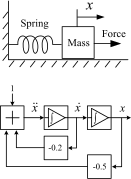
\includegraphics[width=\linewidth]{numerics-ast/AnalogComputerExampleCircuit.pdf}
	\caption[Sketch of a simple analog computing problem.
	\modifiedAfter{AnalogNingPhd}]%
	{Sketch of a damped oscillation as a toy problem from classical mechanics,
		described by the ODE IVP $\ddot x = -0.2 \dot x - 0.5 x + 1$ with ID $x(0), \dot x(0)$.
		The lower panel shows the electrical circuit to solve the \emph{analogue} problem.
		Adopted from \cite{AnalogNingPhd}.}\label{fig:analog-computer}
\end{marginfigure}
While analog computers disappeared from the frontline of computing in favour
of digital computers, even today there is active research stating that analog
computers could solve PDEs in a parallel and energy-efficient way, as it is
out of reach for digital processors \cite{ulmann2013analog}.
It is likely that analog computing will enjoy a similar revival as vector
computing did, in terms of an integration in modern computer generations.
Analog parts could be casted as coprocessors or accelerator
units in the same way as graphic cards and dedicated computing cards are
used today.

In fact, analog models of gravity is a research field on its own
\cite{Barcelo2011,Balbinot:2006ua}, where modern attemps date back to 1980s
proposals of Unruh about accessing black hole evaporation in fluid flows
determined by analog laws \cite{Unruh81}. However, general relativity was not 
solved on analog computers yet, and this remains a research program for the
future.

\section{Time and Space discretizations}
After the excursion of section~\ref{sec:solving-pdes-computers}, for the rest 
of this work, all PDEs are subject to a \emph{numerical} solution (if not 
mentioned otherwise).
This requires to discretize the continuum problem in a suitable way.
The classical literature distinguishes between temporal and spatial
discretization\footnote{
 Where the ``temporal'' direction (dimension) is characterized by the
 (volatile)
 evolution direction while the ``spatial'' directions (dimensions) define
 the spatial simulation domain which is hold in memory.
}.
This section is a short survey in basic grid based methods with focus on
``semi-discrete'' time integration techniques in order to solve PDEs
such as \eqref{intro:ncp}. In contrast, the subsequent
Sections \vref{sec:fv} and \vref{sec:dg} cover fully discrete techniques, \ie
approaches which allow for the PDE solution in a single (uniform) spatial and
temporal discretization procedure.

\subsection{Semi temporal discretization}\label{sec:time-and-mol}
A scheme with spatial discretization, but without a similar
(explicit) temporal one is called \emph{semi discrete}.
Semi discretization is a popular term in literature and may be misleading:
In a numerical attempt to solve PDEs, evventually both the spatial and the
temporal dimensions must be discretized.  However, the different
treatment of the temporal and spatial differential operators as well as the
non-discretization in temporal direction between discrete timesteps
(Figure~\ref{fig:mol})
is a motivation to adopt the term ``semi discrete''.
  
The \emph{method of lines} (MoL) is a particular example of a semi
temporal method. The idea in MoL is 
to recast the PDE describing $u_k(x_i,t)$ into  $n\times N$
ordinary differential equations (ODEs), with $n$ the
state vector length and $N$ the number of points $x_i$ covering the spatial domain
$\Omega$\footnote{
	Note that the MoL approach is invariant under the spatial discretization.
	It does not require any particular grid.
}. That is, the MoL solves one ODE in time (from initial data $t_0$ to $t_1$) 
for every (discretized) spatial point and field, that could be denoted as
\begin{equation}\label{eq:mol-ode}
\partial_t u_k(x_i, t) = \mathcal R(x_i, u_k(t_0), \partial_j u_k(t_0))
\end{equation}
where the spatial differential operator $\mathcal R$ collects all PDE terms
of \eqref{intro:ncp}.
Popular ODE time integrators are Euler's method or the higher order nonlinear
total-variation diminishing (TVD) or 
strong stability preserving (SSP) Runge-Kutta (RK) methods (see
Appendix~\ref{sec:apx-pde-classification} for details). These are explicit
(dependency at time $t$ only on $t_0 < t$, not $t_1 > t$) single-step
(no dependence on $t<t_0$) methods and easy to implement. 
Another popular example for ODE integration are linear multistep high order
integrators, such as the Adams-Bashforth (AB) method which represents the field
with polynomials in time.
The cost to pay for high order methods is the need for repeatedly
evaluate/update the right hand side (RHS) in \eqref{eq:mol-ode},
which requires evaluating spatial
derivatives, which implies communication.

\begin{marginfigure}
	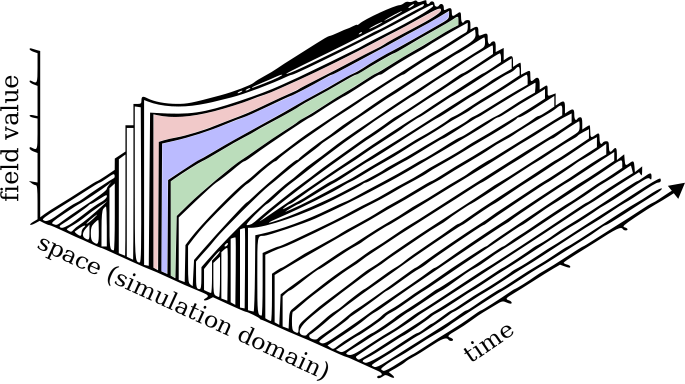
\includegraphics[width=1.05\textwidth]{numerics-mol/mol-motivation.pdf}
	\caption[MOL figure, \colorizedAfter{Schiesser2009}]
	{   Motivation for the naming \emph{Method of Lines}
		\eqref{eq:mol-ode}: The lines are the
		individual solutions at certain positions within the spatial domain,
		over the simulation time. This figure illustrates that space is 
		discretized
		but time is not. The three coloured lines (``slices'' in the 
		height-elevated plot) are neighboured: In order to determine the
		time evolution of the blue slice, information from the green and
		red slice have to be taken into account.
		
		The example shows a scalar diffusion equation $\partial_t \phi = \kappa 
		\partial_x^2 \phi$ 
		with arbitrary $\kappa$ and initial field $\phi_0=\frac 12 
		\exp\left\{-(x-1)^2 
		+ \exp(-(x+1)^2)\right\}$. It is modified and 
		colorized from \cite{Schiesser2009}.
		% Also at english wikipedia: 
		%https://en.wikipedia.org/wiki/Method_of_lines
	}\label{fig:mol}
\end{marginfigure}

Implicit or backward methods such as the Crank-Nicholson are poular for stiff
PDEs due to their small domain of dependency
(\ie the spatial region which influences the solution at a given point due
to causality / characteristic speeds) or for when the timestep size is
constrained by a spatial discretization method (such as in the Discontinous
Galerkin method, see below).
Implicit methods allow larger time\-steps compared to explicit methods. On
the other hand, the solution for a time $t$ has to be found by solving an
implicit equation (\eg iterative root finding).

For special problems, sophisticated time integrators beyond the MoL exist
which take particular problem properties into account. For instance, a
symplectic integrator scheme conserves the momentum space volume $\d p\ \d q$
during the integration of Hamilton's equations by evolving the coupled
canonical coordinates $p$ and~$q$.

\subsection{ADER time integration}
The ADER technique (from \emph{A}rbitrary high order \emph{DER}ivatives) was
pionieered by Toro and Titarev \cite{Titarev2002, Titarev2005, Toro2006}
in the context of Finite volume schemes (Section~\ref{sec:fv}). It
bases on the idea of tayloring the time evolution in~\eqref{eq:mol-ode},
\begin{equation}\label{eq:ader-mol}
\partial_t u_k(x_i, t) = \sum_{l=0}^N \frac{t^l}{l!}
  \partial_t^l u_k(x_i, t_0) \,,
\end{equation}
so that $\Delta t = t-t_0$, and then expressing the $l$th order temporal
derivative with spatial derivatives which are obtained by the PDE weak form
and partial integration with a $N$th order test function, similar as it
will be presented in Section~\ref{sec:dg}. This way, the time update relys on
the $N$th order spatial discretiation and can be computed analytically to $N$th
order.

The ADER approach leads to arbitrary high-order accurate fully discrete one-step
schemes in space and time. The arbitrariness here is just represented by the
fact that $N\in\mathbb N$ can be choosen freely (with bigger $N$ resulting
in higher computational cost, of course). \emph{one-step} effectively means
no repeated evaluation of the \eqref{eq:ader-mol} RHS. This is the
communcation-avoiding property of the ADER approach which pays off on massively
parallel grids.\footnote{
	Appendix \vref{sec:rkdg-performance} compares the ADER time evolution with
	the Runge-Kutta one.
	
}

%\todo{hier komischer Verweis auf Astrophysik-Verewendungen, weiß nicht ob das
%gut ist}
%ADER schemes have already been applied to the
%equations of relativistic MHD, both in the ideal case (see
%\cite{Dumbser2008,Zanotti2015,Zanotti2015d}) and in the
%resistive case \cite{Dumbser2009} and to other nonlinear
%systems of partial differential equations
%\cite{Zanotti2015c,Fambri2017}.

\subsection{CFL factor}
In hyperbolic systems, the temporal discretization is limited by the spatial
discretization. The formalization for limiting the timestep size
$\Delta t = t_1-t_0$ is known as the Courant-Friedrichs-Lewy (CFL) condition.
The argument can easily derived by the classical kinematic law
$s=v\cdot t$, with $s$ the traveled
distance of a particle moving with constant velocity $v$ over time $t$.
Given the distance $\Delta x = \Lambda_i \Delta t$ is traveled by a system's
wave with characteristic (eigenvalue) $\lambda_i$, the maximum timestep is
therefore constrained from above,
\begin{equation}\label{eqn:def-cfl}
\Delta t \leq \Delta x / \Lambda \,,
\end{equation}
with $\Lambda$ the maximum of the systems eigenvalues $\lambda_i$. In practice,
the inequality \eqref{eqn:def-cfl} is replaced by
$\Delta t = C \Delta x / \Lambda$ with $0 < C \leq 1$, where the arbitaryily
chosen $C$ is called the CFL or Courant factor.

\subsection{Methods for spatial discretization}
For spatial discretization, there exist a couple of standard classes with 
different attemps.
While adopting a somewhat regular grid (Figure \ref{fig:fd-stencil-intro}) is
probably obvious (Section \ref{sec:grid-meshing} discusses grid meshing in detail),
there is a whole class of \emph{meshfree} methods. A particular example is
smoothed-particle hydrodynamics (here coordinates move with the fluid), which is
in particular popular in astrophysics, since it easily allows to
cover several orders of magnitude in length scales. Hybrid attemps exist, such
as Particle-in-cell (PIC) approaches which combines particle methods with
grid based ones.

Another general class of methods are \emph{spectral} methods where the simulation
domain $\Omega$ is covered by a function basis \cite{hesthaven2007}.
This is typically used for smooth
problems where Fourier series can be used to eliminate differential operators.
Formally, spectral methods belong to \emph{finite element} methods (FEM) which first
subdividide the computational domain $\Omega$ by a finite number of (typically)
nonoverlapping elements $\Omega_i$ where the spectral methods are then applied
within (see also Section~\ref{sec:dg-subcell-structure}). 
Finite-element methods are
known also under the name of {variational-difference} or
{projection-difference} methods \cite{Ritz1909,Galerkin1915}.

\emph{Finite volume} methods (FVM or just FV) share some features with FEM,
and these two terms can be used in some respect synomyously, whereas ``FEM''
has a slight focus on meshing topologies and embedding of methods within
single cells, while ``FVM'' has to some extend a focus on the integral
formulation and interfacing of cells (Godunov's method, Riemann problem),
typicall implemented around a grid with small volumes around spatial points.

A clear distinction however can be made between FV and \emph{finite 
differences} (FD) methods. In the later method, the PDE is solved by employing
the finite difference quotient between certain connected points in a grid,
while a FV scheme works on volume and surface integrals, applying Gauss'
theorem.

\subsection{Finite-difference schemes}
\begin{marginfigure}[-4cm]
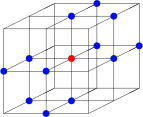
\includegraphics[width=\linewidth]{numerics-schemes/FD-Stencil-3d.pdf}
\caption[
  FD stencil motivational cartoon, \colorizedAfter{FDStenicl3d} 
]{
  Example of an arbitrary three dimensional finite differencing stencil.
  Dependent points (blue) are neighbouring the evaluation point (red).
  In order to compute the derivative of a field on this grid at the red point,
  all dependent points in a certain direction projection are taken into account.
  (coloured from \cite{FDStenicl3d})
}\label{fig:fd-stencil-intro}
\end{marginfigure}

Finite differencing is probably the most straightforward way of solving
differential equations on a computer. The starting point and origin of
the name is to undo the infinite limit $h\to\infty$ of the difference quotient
\begin{equation}
\dd{f(x)}{x} \approx \frac{f(x+h) - f(x)}{(x+h) - x}
\end{equation}
By choosing a finite but small $h$, the spatial differential operator in the
Method of Lines \eqref{eq:mol-ode} can be computed. The most simple way to
implement this is to discretize space on a finite number of grid points
$x_i = i\Delta x$, store the
function values $f(x_i)=f_i$ and set $h=\Delta x$.

The concept is easily extended to generic finite differencing stencils
(Figure~\ref{fig:fd-stencil-intro}),
higher dimensions and arbitrary order derivatives ($\d f/{\d^n x}$).
%Adopting finite differencing codes for solving hyperbolic conservation laws
%have a long tradition.
Finite differencing techniques are popular for being computationally cheap
and easy to implement. For instance, there is no need to cast a PDE system
into a particular form (such the nonconservative form \eqref{intro:ncp}) and
rectangular regular grids as well as differential stencils
can be represented by (continous storage) arrays.

\begin{marginfigure}[-2cm]
\includegraphics[width=\linewidth]{ghost-cells-ratio/ghost-cell-ratio.pdf}
\caption[
  Sketch of the ghost cell ratio to payload ratio, \exclusive
]{
  Ghost cell volume $G=12xw^2 + 6x^2 w + 8w^3$ to actual physical
  domain $V=x^3$ ratio $R=G/V$ in three dimensions for
  different ghost layer widths $w$ (\ie half the stencil sizes in FD context).
  On the abscissa, the width $x$ of a cuboid (domain or patch) is given in
  number of cells. These small patches are realistic in the
  \code{ExaHyPE} AMR code, while traditional codes such as \code{Cactus}
  have an order of magnitude larger cells.
}
\label{fig:ghost-cell-ratio}
\end{marginfigure}

A major drawback of obtaining high order in a large simulation is the
appearance of \emph{ghost points} outside the simulation domain. In a naive
cartesian domain decomposition for the parallel evaluation of the
differential operator, the ``ghost halo'' fraction can quickly make a
substantial part of the simulation domain on the computer which is especially
costly when it comes to data exchange in the boundary
(Figure~\ref{fig:ghost-cell-ratio}).%

A numerical drawback of high order finite differencing schemes is the 
unsuitability for discontinous solutions where the large stencil will generate
spurious solutions. This makes them unattractive for nonlinear conservation
laws. On the other hand, such problems do not occur in linear and linearly
degenerate systems\footnote{In section \vref{sec:fo-ccz4} it will be shown
that parts of a  particular formulation of Einstein equations, the CCZ4
equations, can be written in a linear degenerate way.} where no shocks can be 
generated if the initial data is not discontinuous itself.

Finite difference methods can be ``fortified'' with a number of methods such
as \emph{artificial dissipation} for stabilisation \cite{Kreiss73}.
Another typical choice
for hyperbolic conservation laws are special \emph{upwinding} stencils to
correctly track the system characteristics. Both topics are typically
covered by Riemann solvers in FV schemes and implementing them explicitely
in FD schemes can be seen as a hardening of the simple FD schemes in order
to gain robustness by maintaining a computationally and logically cheap scheme.
In the same way, FD can also be used empowered
with high resolution shock capturing (HRSC) techniques.
\todo[color=green]{
  FD schemes: There are many details which could be added, such as dissipation
  stencils; citations about Upwinding, HRSC, etc.
}

% Further papers:
%          FD in NR \cite{Baumgarte2010,Bona2009}
%          interesting outlook: Compact finite differences \cite{Lele92}

\section{Finite-volume schemes}\label{sec:fv}
\begin{marginfigure}[2cm]
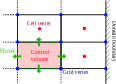
\includegraphics[width=\linewidth]{numerics-schemes/FV-Cells.pdf}
% Roughly inspired by 
% \url{http://arturo.imati.cnr.it/~marco/Research/Finite_Volumes/index.html}
\caption[
   Cartoon of a Finite Volume description, drawn with Inkscape, \exclusive
  ]%
  {Finite volume simulation domain and termiology in an exemplaric simple
   two-dimensional Cartesian grid with rectangular cells. Shown are the cell
   barycenters, the cell corners, a domain boundary, the fluxes/waves which
   are described by the Riemann problem for a single highlighted
   demonstrator cell.
}
\end{marginfigure}

Finite-Volume schemes discretize the simulation domain $\Omega$
into cells $\Omega_i$ which shall hold \emph{cell averaged} or
\emph{piecewise constant} solutions. It was the insight of Godunov
in 1959 \cite{Godunov59} to solve then the Riemann problem (Section~\ref{sec:riemann-problem})
at these interfaces in order to solve the PDE. Godunov's method itself is
fully discrete in time and space, but its time update can easily be replaced
by the method of lines (Section~\ref{sec:time-and-mol}).
%With this approach, the problem of
%solving the RHS of MOL reduces to the interfaces $\partial\Omega_i$
%between these cells and it was the insight of Godunov in 1959 to solve the
%Riemann problem at these interfaces
For recent reviews for FV in relativistic astrophysics, see \cite{Font08,Marti03}.

\subsection{Godunov's scheme}
A finite volume scheme works on the average value $\u^n_i$ of the state vector within
a spacetime-cell $[t^n, t^{n+1}] \times \Omega_i$, and for simplicity we work in
one dimensions in this subsection, so $\Omega_i=[x_i, x_{i+1}]$,
$\Delta t = t^{n+1} - t^n$ and $\Delta x=|\Omega_i|=x_{i+1}-x_{i}$. The cell barycenter is located at $x_{i+1/2} = x_i + \Delta x/2$ and the cell average given by
\begin{equation}
\label{eqn.subcellaverage}
\bar \u^n_i := \frac{1}{|\Omega_i|} \int \limits_{\Omega_i}
\u(t^n,x)  ~\d x
\,.
\end{equation}
Godunov's scheme can be derived by integrating the PDE \eqref{intro:ncp}
in time and applying the piecewise constant assumption $\u(t,x) \equiv \u_i^n$
for $t\in[t^n,t^{n+1}]$. The time integral collapses and allows to write
\begin{equation}\label{eq:godunov}
\u^{n+1}_i = \u^n_i - \frac{\Delta t}{\Delta x}
   \left(\boldsymbol f_{i+1/2} - \boldsymbol f_{i-1/2} \right)
   + \frac{\Delta t}{\Delta x} \boldsymbol B \cdot
   \left( \u^n_{i+1/2}  - \u^n_{i-1/2} \right)
   + \Delta t \boldsymbol S(\u^n_i)
   \,.
\end{equation}
Here, a couple of remarks are neccessary: First, this scheme is obviously
fully discrete in space and time, as well as explicit in time. The conserved
flux was replaced by a numerical flux which is thanks to the piecewise
constant assumption just given as
%Analytically the numerical flux is a time integral over the cell surface,
%\begin{equation}\label{eq:godunov-flux-integral}
%\boldsymbol f_{i\pm 1/2} =  \int\limits_{t^n}^{t^{n+1}} \frac{\d t}{\Delta t} \boldsymbol F(\u(t,x_{i\pm 1/2}))
%\end{equation}
%however,allows the integral \eqref{eq:godunov-flux-integral} to collapse and the fluxes
%to be given just as
\begin{equation}
\begin{aligned}
\boldsymbol f_{i - 1/2} &= 
 \frac 12 \left(
 \boldsymbol F(\u^-_{i-1/2}) + 
 \boldsymbol F(\u^+_{i-1/2})
 \right)
&&=
\frac 12 \left(
   \boldsymbol F(\u^n_{i-1}) + 
   \boldsymbol F(\u^n_{i})
\right) \,,
\\
\boldsymbol f_{i + 1/2} &= 
\frac 12 \left(
 \boldsymbol F(\u^-_{i+1/2}) + 
\boldsymbol F(\u^+_{i+1/2})
\right)
&&=\frac 12 \left(
\boldsymbol F(\u^n_{i+1}) + 
\boldsymbol F(\u^n_{i})
\right) \,.
\end{aligned}\label{eq:godunov-riemann-trivial}
\end{equation}
Second, since Godunov's method is first order, the nonconservative contribution
vanishes as the boundary extrapolated data are equal, $\u^n_{i+1/2}  - \u^n_{i-1/2}=0$.
The nonconservative source term $\boldsymbol B$ therefore vanishes.

The essential idea of Godunov is now that with the piecewise constant assumption,
a Riemann problem can be solved at each cell interface. The initial data for the
Riemann problem between $x_{i}$ and $x_{i+1}$ is then given by the two cell values
\begin{equation}\label{eq:godunov-riemann-interface}
\u(t^n,x) = \u^n_i \theta(x-x_{i+1/2}) + \u^n_{i+1} \theta(x_{i+1/2}-x)
\end{equation}
with Heaviside step function $\theta(z)$.
Once the Riemann problem is solved, also
the the time update \eqref{eq:godunov} is given
\footnote{
 The CFL conditions \eqref{eqn:def-cfl} must be fulfilled and the scheme can be
 easily extended to higher dimensions in a dimension-by-dimension fashion.
}. We call equations of type
\eqref{eq:godunov-riemann-trivial} Riemann solvers and in fact this simple one
is already sufficient for first order Godunov. However, there are more sophisticated
Riemann solvers which do not make the piecewiese constant assumption. 
Popular choices are the Roe solver and HLLE solver (see next Sections).

\subsection{Higher order finite volume}
\begin{marginfigure}
	\centering
	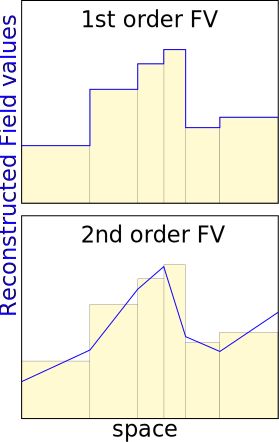
\includegraphics[width=0.88\linewidth]{exahype-2nd-order-fv-gridstructure/high-order-reconstruction.pdf}
	\caption[FV Higher order reconstruction, Cartoon drawn with Inkscape, 
	\exclusive]%
	{Cartoon which demonstrates how higher order reconstruction of the field
	 works: While a first order reconstruction method assumes cells to have
	 an average value (cells in this one-dimensional example are non-uniformly
	 sized), in a second order reconstruction (think of a Taylor expansion in
	 each cell, with a linear term) the field is approximated by taking
	 neighbouring cells into account. In general, requirements such as a
	 continuity condition do not neccessarily have to be fulfilled, while
     they typically are desirable in schemes.
     }
	\label{fig:higher-order-reconstruction}
\end{marginfigure}
Higher order FV is archieved by improving description of the interface
state values $\u^{\pm}$ by taking next-to-neighbour cells into account. 
The simplest
possibility is to switch to a piecewise linear 2nd order description
where $\u_i(x) = \u_i + v_i(x-x_i)$ within a cell 
(Figure~\ref{fig:higher-order-reconstruction}).

TVD conditions lead to non-linear limiting of slopes, such as the minmod limiter.
In general, a $k$th order reconstruction operator
\begin{equation}
\mathcal R\left[ \q_i \right] = \lim_{y \to x_i} \q(y) + \mathcal O(\Delta x^k)
\end{equation}
applied at a cell average at position $x_i$ reconstructs the continous field $\q$
locally around $x_i$. Successful methods used in the literature are for
instance the
piecewiese parabolic method (PPM), the essentially non-oscillatory (ENO),
the weighted essentially non-oscillatory (WENO) and the monotonicity-preserving 
(MP) \cite{Radice2012b}.
All of them are high resolution shock capturing, \ie they preserve a good resolution
at discontinuities and do not introduce spurious oscillations.

Similar as to FD methods, for a $k$th order reconstruction, the domain of dependency
includes $k$ neighbouring cells per dimension. Reconstruction operators can also be
formulated in stencils which look like FD stencils.

\subsection{Riemann solvers and the nonconservative 
product}\label{sec:riemann-nonconservative}
The generic integral form for solving \eqref{intro:ncp} with FV introduces a space
and time integral,
\begin{fullwidth}
\begin{equation}
\label{eqn.fv.generic}
\boldsymbol{u}^{n+1}_{i} - \boldsymbol{u}^{n}_{i} 
%
- \iint \limits_{T^n ~ \partial\Omega_i}
\mathcal F(\q^-,\q^+)
\,\mathrm d^d x\,\mathrm dt
= \iint \limits_{T^n ~ \Omega_i}
\left[\boldsymbol S(\q) - \boldsymbol{B}(\q) \cdot \nabla \q  \right]
\,\mathrm d^d x\,\mathrm dt
\,.
\end{equation}
\end{fullwidth}
Here, $\mathcal F$ is the numerical flux at the element interface. If not mentioned
otherwise, a simple Rusanov Riemann solver is used \cite{Rusanov1961a},
\begin{fullwidth}
\begin{equation}
\mathcal{F}\left(\q_h^-, \q_h^+ \right) \cdot \boldsymbol{n} = \frac{1}{2}
\left( \boldsymbol{F}(\q^+) + \boldsymbol{F}(\q^-) \right) \cdot \boldsymbol{n}
- \frac{1}{2} |\Lambda_i| \left( \q^+ - \q^- \right) \pm \frac 12 \boldsymbol 
B\left( \frac{\q^+ + \q^-}2 \right)
\cdot \boldsymbol{n} \left( \q^+ - \q^- \right)\,.
\label{eq:rusanov}
\end{equation}
\end{fullwidth}
Note that for the piecewise constant approximation (Godunov's first order scheme),
$\q^+ = \q^-$ and \eqref{eq:rusanov} reduces to 
\eqref{eq:godunov-riemann-trivial}.

It should be stressed that the use of the nonconservative product within the
Riemann solver/path conservative integration is \emph{not} required per-se.
It would have been equally possible to integrate a differential source in a
non-path conservative way. However, the special treatment allows it to formulate
well-balanced numerical methods \cite{Bermudez1994}. 

%\todo{Important: Move NCP discussion from ADER-DG scheme to this point}
The inspiration to use {path-conservative} schemes for
nonconservative products has been taken from successful developments in
the context of  {well-balanced} numerical methods
for the solution of the shallow-water equations 
\cite{Pares2006,Castro2006,Castro2010},
where the bottom-slope term (which is the gradient of a known
function and accounts for gravitational forces in shallow-water models) is 
discretized as a nonconservative product in the principal part of the
system rather than as a classical algebraic source term. In the shallow
water context, the family of path-conservative schemes allows to preserve
certain stationary equilibrium solutions {exactly} up to machine
precision also on the discrete level, including nontrivial equilibria
\cite{Gaburro2017,Gaburro2018}.


%In the following, a MUSCL TVD scheme as well as a WENO shall be presented in detail,
%as they are implemented in ExaHyPE.

\subsection{MUSCL-Hancock}\label{sec:MUSCL}
\begin{marginfigure}[3cm]
	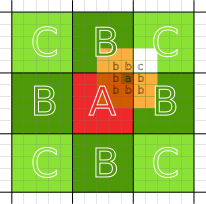
\includegraphics[width=\linewidth]{exahype-2nd-order-fv-gridstructure/exahype-2nd-order-fv-gridstructure.pdf}
	\caption[2nd order FV ExaHyPE ghost cell problem, drawn with Inkscape, 
	\exclusive]%
	{
       Cartoon of the ghost cell optimization in \code{ExaHyPE}:
       Patches are denoted with upper case letters ($\mathbb A$, $\mathbb B$,
       $\mathbb C$), while embedded FV subcells are denoted with lowercase
       letters ($\mathbb a$, $\mathbb b$, $\mathbb c$). The letter $a$ refers
       to the patch/cell which solution shall be computed. The letters $b$
       refer to their direct neighbours (sharing a face), while the letters
       $c$ refer to the corners (sharing an edge).
       Two ghost layers are drawn.
       Here, the information in the domain $\mathbb C \cap \mathbb c$ is
       not available.}\label{fig:muscl-exahype}
\end{marginfigure}

The second-order acurate MUSCL-Hancock TVD finite-volume scheme
\citep{toro-book} is the second-order FV scheme available in
\code{ExaHyPE}. It has proven robustness in the presence of
shock waves and low density atmospheres. 
Formally, the second-order MUSCL-Hancock scheme can be derived from the PDE
\eqref{intro:ncp} as in \eqref{eqn.fv.generic}.

High order in space, together with non-oscillatory properties, are
achieved  via a {nonlinear} reconstruction of
piecewise polynomials from the known cell averages
$\bar{\boldsymbol{v}}_{i,s}^n$ using a TVD reconstruction. In order to
preserve high resolution shock capturing properties, high order
reconstruction requires slope limiting (also refered to as flux limiting).
Such a limiter allows to restrict the order of the scheme at discontinuities.
In \code{ExaHyPE}, different slope limiters were implemented, such as the
\emph{minmod} \cite{Roe86} or the \emph{Koren} limiter~\cite{Koren1993}.

Particulary relevant for \code{ExaHyPE} is the fact that in this code,
the reconstruction stencils at patch boundaries lack isentropy
(Figure~\ref{fig:muscl-exahype}).
In \code{ExaHyPE}, corner cells are not synchronized for performance reasons
(especially because it is primarily a DG code and DG does not require
the knowledge of corner values). This requires the FV reconstruction in
$d\geq 2$ dimensions to stick to a $+$ shaped stencil at the corner
(domain $\mathbb A \cup \mathbb B$ or $\mathbb a \cup \mathbb b$ in Figure
\ref{fig:muscl-exahype}), \ie the field information $\mathbb c$ is not
available, while $\mathbb B$ and $\mathbb b$ is.
For slope limiting, a conservative estimate (guess) on the slopes has to be
made.
The problem does not occur in a first order scheme where no
reconstruction takes place.

\subsection{WENO}

As an alternative to the MUSCL scheme, an arbitarily accurate ADER-WENO
finite-volume schemes can be used in the \code{ExaHyPE} prototype.
The weighted essentially non-oscillatory (WENO) approach does not clip local
extrema, in contrast to the second-order TVD method. For fluid dynamics
(Chapter~\ref{chapter:hydro}) the TVD scheme was found to be more robust
than the WENO scheme.

The (ADER-) WENO scheme scheme shares many aspects of the (ADER-) DG
schemes presented in the subsequent Section~\ref{sec:dg}. The spacetime
predictor solution $\q_h$ is however computed from an initial
conditition given by a WENO reconstruction polynomial $\w_h(\x,t^n)$
computed from the cell averages
$\bar{\u}^n_{i,s}$ via a multi-dimensional WENO reconstruction operator
detailed in \cite{Jiang1996,Dumbser2008,Dumbser2013}. The values at the cell
interfaces $\q_h^-$ and $\q_h^+$ are computed as the boundary
extrapolated values from the left and the right subcell adjacent to the
interface.

The nonlinear WENO reconstruction works as follows: for each subcell
$\Omega_{i,s}$ we compute several reconstruction polynomials
$\w_h^k(\x,t^n)$ requiring integral conservation of $\w_h^k$ on a set of
different reconstruction stencils $\mathcal{S}^k_{i,s}$,% \ie
\begin{equation}
\frac{1}{|\Omega_{i,j}|} \int \limits_{\Omega_{i,j}} \w^k_h(\x,t^n)
d \x = \bar{\u}^n_{i,j} \qquad \forall \, \Omega_{i,j} \in
\mathcal{S}^k_{i,s}\,.
\end{equation}
This system is solved via a constrained least-squares algorithm requiring
at least exact conservation in the cell $\Omega_{i,s}$ itself 
\cite{Dumbser2007b}. From the set of reconstruction
polynomials $\w_h^k$, the final WENO reconstruction polynomial $\w_h$ is
obtained by using a classical nonlinear weighted combination of the
polynomials \cite{Jiang1996,Dumbser2007b}
%
\begin{equation}
\label{eqn.weno}
\w_h(\x,t^n) = \sum \limits_k \omega_k \w_h^k(\x,t^n),
\quad \textnormal{with} \quad \omega_k = \frac{\tilde{\omega}_k}
{\sum \limits_l \tilde{\omega}_l}
\quad \textnormal{and}  \quad \tilde{\omega}_k = \frac{\lambda_k}
{(\sigma_k + \epsilon)^r}\,,
\end{equation}
%
where the oscillation indicators $\sigma_k$ are computed from
%
\begin{equation}
\sigma_k := \sum \limits_{l\geq 1} \int \limits_{\Omega_{i,s}}
\Delta \x_{i,s}^{2l -1} \left( \frac{\partial^l}{\partial \x^l}
\w_h^k(\x,t^n) \right)^2 d \x\,.
\end{equation}
%
The small parameter $\epsilon$ in \eqref{eqn.weno}, which is only
needed to avoid division by zero, is typically set to $\epsilon=10^{-14}$
and the
exponent in the denominator is chosen as $r=8$. The linear weights are
$\lambda_1 = 10^5$ for the central stencil (\ie $k=1$), while all other
stencils (\ie $k>1$) have linear weight $\lambda_k=1$. This choice
corresponds also to the one made in \cite{Dumbser2007b}.

In a practical implementation it is convenient to write also the
WENO reconstruction polynomials in terms of some reconstruction basis
functions $\psi_l(\x)$ as $\w_h(\x,t^n) = \Psi_l(\x) \hat{\w}_l^n$. 
Here, following \cite{Dumbser2008}, the basis functions $\Psi_l$
are defined in the same way as the $\Phi_l$ in Section~\ref{sec:dg-subcell-structure},
\ie as tensor products of Lagrange
interpolation polynomials through the Gauss-Legendre quadrature
nodes. %For the limiter, we only use a piecewise quadratic reconstruction,
%leading to a nominally third-order accurate scheme. As already mentioned
%before, the predictor is computed according to \eqref{eqn.pde.st2}, where
%the initial data $\u_h(\x,t^n)$ is replaced by $\w_h(\x,t^n)$ and the
%spatial control volumes $\Omega_i$ are replaced by the subcells
%$\Omega_{i,s}$.

\section{Discontinous Galerkin schemes}\label{sec:dg}
\begin{marginfigure}[-4cm]
  \includegraphics[width=\textwidth]{dg-fv-intro-sketch/fileformat-sketch-cont.pdf}
  \includegraphics[width=\textwidth]{dg-fv-intro-sketch/fileformat-sketch-discont.pdf}
  \caption[
    1D DG Motivational example, Matplotlib sketch, 
    \publishedIn{exahype-guidebook}
  ]{A motivational cartoon of DG in one dimensions: A $N=2$ polynomial
    with $N+1$ DOF ($a+bx+cx^2$) is embedded in each cell. The cell sizes and
    nodal basis points (red) are arbitrary in this plot and in general. The
    shading indicates the single cell averages (one DOF). The upper panel shows
    a continuous function while the lower panel shows an example with 
    jumps/discontinuities at the cell interfaces, yielding in a double valued
    function at the cell interface. In contrast to high order FV, the DOF
    really live within a single cell and no reconstruction takes place which
    averages over multiple cells.}
  \label{fig:dg-motivational-sketch}
\end{marginfigure}

Galerkin methods (developed independently by Boris Galerkin and Walther Ritz,
but named only after Galerkin)
are another method to discretize a PDE, by casting it in a weak (integral)
formulation
where test function and solution are part of a Hilbert space. A finite
discretization is then achieved by the approximative projection to a
finite-dimensional Hilbert space; a matrix representation instead is achieved
by finding an orthogonal basis in this function vector space. Formally this
class of methods bear resemblance to spectral methods and can share the same
properties such as exponential convergence. Thus Galerkin methods are formally
finite element methods which combine the advantages of spectral methods with
grid-based methods.

Discontinous Galerkin (DG) schemes then again combine Galerkin methods with
Finite Volume paradigms (Godunovs methods). DG methods can be motivated as
an extension to FV methods where a single cell average is replaced by more
degrees of freedom, such as a linear or quadratic approximation of the real
solution. As the particular feature, the approximations between the cells
don't have to be smooth/continous but can exhibit jumps
(Figure~\ref{fig:dg-motivational-sketch}). Of course, in the continuum limit
where the cell size goes to zero while the number of cells goes to infinity,
these discontinuities are as well defined as the discontinuity of Godunovs
piecewise constant method itself.

Given the concept of embedding information within a cell (or patch), DG methods
exhibit $hp$-adaptivity: Meshes can be refined both in terms of cells
($h$-refinement) or in terms of subcell degrees of freedoms ($p$-refinement).
For classical grid $h$-refinement, DG methods exhibit polynomial accuracy
(similar to FV/FD), while for subcell $p$-refinement they exhibit spectral
accuary.

In DG methods, the number of degrees of freedom $p$ is naturally associated to
the order of the scheme. A major benefit of DG schemes is the need of only one
ghost layer \footnote{
  Since DG uses a polynomial basis, the concept of an integral number of
  ``layer cells'' (as in FD/FV) makes no sense. One ghost layer means, that
  the field values on the lower-dimensional surface of the computational domain 
  need to be exchanged within the corrector phase of the scheme presented
  in Section~\ref{sec:holy-dg-scheme}. In a two dimensional simulation on
  square elements, the one dimensional polynomials on four element border lines
  have to be exchanged. In a three dimensional simulation on cuboid elements,
  the two dimensional polynomials on six element surfaces have to be
  exchanged. No particular treatment is neccessary for the edges/corners of
  the squares/cuboids.
} at any order, due to the functional basis within one cell. That
provides optimal scalability and makes DG attractive for large parallel 
problems,
in fact explains the spreading of DG methods in the Exascale era. The price
which has to be paid (in comparison to a FV scheme) is primarily the complexity
of an implementation which cannot be underestimated. The DG method will get
intertwined with the way how the grid is managed and how communication works.
Arguable disadvantges of the DG method (compared to a FV method) are its
apparently larger memory footbringt, coming from the larger amounts of degrees
of freedom and, for explicit DG methods, the limitation on the timestep size (a
penalty of $\sim 1/2N$
where $N$ is the degrees of freedom, compared to a FV method). However, this
criticism disregards the high order spectral convergence which allows to
describe smooth problems with orders of magnitudes less cells then any high
order FV method would allow to. A way to alleviate the severe CFL timestep
restriction is the use of semi-implicit DG schemes, as those proposed, for
instance by \cite{Tavelli2016,Fambri2016}.

DG methods have been proven to be non-linearly stable at all orders and can
be formulated covariantly~\cite{meier_1999_mas}. Similar as Godunovs method, the
mathematical foundations are only well defined for first order PDEs,
but DG has been applied to second order PDEs.

It has taken nearly two decades for the DG methods to be
extended to general nonlinear hyperbolic systems, thanks to the
groundbreaking works of \cite{Cockburn1989b,Cockburn1990,CockburnShu98}.
DG methods are reviewed in 
\cite{cockburn_2000_dg,cockburn_2001_rkd,Shu2016,hesthaven2007,hesthaven2008,Cockburn2003}
whereas \cite{ADERNSE,Dumbser2009,Dumbser2010b} provide the fundaments
for the path-conservative nodal semi-discrete ADER-DG methods which are
presented in the following.
%

\subsection{Subcell structure in nodal DG schemes}\label{sec:dg-subcell-structure}
In order to mathematically describe the DG structure, a couple of symbols
shall be introduced. The
computational domain $\Omega$ is fully covered by a finite number $N_e$ of 
non-overlapping elements $\Omega_i$, also referd to as \emph{patches} or 
\emph{cells}  \cite{Khokhlov98}. Especially
the usage of the term \emph{cells} stresses the close relationship to FV 
methods. 
In $d$ spatial dimensions, the cells are characterized by their individual size
$\Delta \vec x_i \in \mathbb R^d$
and barycenter $\vec x_i \in \mathbb R^d$.
%
The discrete solution (state vector of the PDE) is denoted by
$\boldsymbol{u}_h$ and is defined in the space of tensor products
of piecewise polynomials of degree $N$ in each spatial direction,~\footnote{
 	To clarify:
 	$\boldsymbol u$ is the analytic solution while $\boldsymbol u_h$ is
 	an approximation within the restricted space of solutions which
 	can be represented by piecewise polynomials.
 	
 	Furthermore, for the sake of a readable notation, vector indices are
 	now neglected in favour of discrete indices and flags.
 } 
\begin{equation}
\boldsymbol{u}_h(\boldsymbol{x},t^n) = \sum \limits_l \hat{\boldsymbol{u}}_{i,l}
\Phi_l(\boldsymbol{x}) := \hat{\boldsymbol{u}}_{i,l}^n \Phi_l(\boldsymbol{x})\,.
\label{eqn.ansatz.uh}
\end{equation}
Here, obviously the spatial basis functions
$\Phi_l(\boldsymbol{x})$ spawn the
orthogonal $N^d$-dimensional function vector space $\mathcal{U}_h^N$. In 
$\mathcal{U}_h^N$,
$\boldsymbol u$ has the components $\hat{\boldsymbol u_l}$ in each direction
$l\in \mathbb N^d$. $\hat{\boldsymbol u_l}$ are the discrete components/degrees
of freedom of the solution which have to be stored.

The spatial basis functions $\Phi_l(\boldsymbol{x}) = \prod_{i=1}^d 
\varphi_{l_i}(\xi_i)$ are generated by the one-dimensional
basis functions $\varphi_k(\xi)$ on a one-dimensional reference element with
normal extend $\xi\in[0,1]$. The physical coordinates $\boldsymbol x\in\Omega_i$
are mapped to the reference coordinates $\boldsymbol \xi\in[0,1]^d$ by
\begin{equation}
\boldsymbol{x} =
\boldsymbol{x}_i - \halb \Delta \boldsymbol{x}_i + \boldsymbol \xi
\cdot \Delta \boldsymbol x
\,.
\end{equation}
\begin{marginfigure}
	\includegraphics[width=\textwidth]{aderdg-subcell-grid-tikz/gauss-lagrangue-grid.pdf}
	\caption[
	  Gaussian quadrature nodal basis examples, TikZ figure,
	  \ownPub{Dumbser2017}.
	]{Some Gaussian quadrature nodal basis on the one-dimensional reference cell.
	  These two examples have been implemented in the \code{ExaHyPE} code.}
	\label{fig:guass-lagranguage-grid}
\end{marginfigure}
In order to apply Gaussian quadrature, typically Legendre polynomials are used
for the basis functions $\varphi_k(\psi)$ and $\xi_i$ shall be the quadrature
nodes of the $(N+1)$ point Gauss quadrature formula. The Gauss-Legendre 
quadrature has the advantage of a diagonal mass matrix \footnote{
  The mass matrix is defined as $M_{ij}=\int \Phi_i(x) \Phi_j(x) \d x$.
  An extensive discussion of the consequences of a non-diagonal Mass matrix and
  especially of Gauss Legendre vs. Gauss Lobotto in AMR codes is given
  in~\cite{Teukolsky2014MM}.
}. The cost to pay is a non-uniform
nodal basis (subcell grid structure), especially there is no nodal point at the
cell boundary\footnote{This hides the double valued character of the field
 value at the patch boundary at the first glance, for instance when no polynomial
 reconstruction is done in a naive (Gauss-Legendre) vertex-interpolating
 visualization, as typically done when vizualizing DG results.}.
In our implementation we also support the Gauss-Lobatto
quadrature with its uniformly distributed nodal points. In this basis, there are
always points on the cell boundary (Figure~\ref{fig:guass-lagranguage-grid}).
The actual nodal basis is a pure technical decision and (except for the
quadrature rule) has no impact on the mathematical structure of the scheme,
therefore we assume the Legendre nodes in the following exposition whenever
in doubt. \footnote{
See also \cite{stroud}
for a detailed discussion of multidimensional quadrature.
}

The orthogonal polynomials satistfy the interpolation property
$\varphi_k(\xi_j) = \delta_{kj}$. Thanks to this nodal tensor product basis, 
the entire subsequent scheme can be written \emph{dimension for dimension}, all
higher-dimensional
integrals decompose in a multiplication of one-dimensional integrals which
can be evaluated on $N+1$ DOF in each dimension. 

To summarize, note again that the
total number of quadrature points $\{\x_{\text{GP}}^m\}$ in
$\Omega_i$, as well as the total number of basis elements $\{ \phi_k\}$,
is $(N+1)^d$.